
% In the plots:
% add points

\chapter{An adaptive implicit midpoint rule time integrator}
\label{sec:adaptive-imr}


The implicit midpoint rule (IMR) is a well known time integration method with a number of favourable properties when applied to standard ordinary differential equations (see \cref{sec:time-discretisation} or \cite[204]{HairerNorsettWanner}).
It also has beneficial ``geometric integration'' properties when applied the Landau-Lifshitz-Gilbert equation (discussed in \cref{sec:ensuring-constant-mv,sec:energy-cons}) and energy conservation properties when applied to the semi-discretised Navier-Stokes equations \cite{Sanderse2013}.
However IMR belongs to the implicit Runge-Kutta family of methods, and as such it is a non-trivial task to create an efficient adaptive time step selection algorithm.
In \thisref{sec:adaptive-imr} we describe a novel adaptive IMR algorithm based on estimates of the local truncation error by a predictor step.


\section{Fixed step size implicit midpoint rule}
\label{sec:fixed-step-implicit}

Let $\yv(t)$ be a vector function and denote an approximation to $\yv(t)$ at $t = t_n$ by $y_n$.
Let $\dtn = t_{n+1} - t_n$ be the $n$th time step (or just ``step'').
Then given a system of ordinary differential equations (ODEs) of the form
\begin{equation}
  \yv'(t) = \ffv{t, \yv(t)},
  \label{eq:43}
\end{equation}
the implicit midpoint rule (IMR) is
\begin{equation}
    \yv_{n+1} = \yv_n + \dtn \ffv{\frac{t_{n+1} + t_n}{2}, \frac{\yv_n + \yv_{n+1}}{2}}.
\end{equation}

We introduce some notation for the midpoint values of $t$ and $\yv$:
\begin{equation}
  \begin{aligned}
    \thf & = \frac{t_{n+1} + t_n}{2} \quad \bigb{= t_n + \frac{\dtn}{2}}, \\
    \yvm &= \frac{\yv_{n+1} + \yv_n}{2}.
  \end{aligned}
\end{equation}
In this notation the IMR is
\begin{equation}
  \yv_{n+1} = \yv_n + \dtn \ffv{\thf, \yvm}.
  \label{eq:basic-midpoint}
\end{equation}

The IMR can also be written in the standard form for Runge-Kutta methods as
\begin{equation}
  \begin{aligned}
    k_1 &= \ffv{t_n + \frac{1}{2} \dtn, \yv_n + \frac{1}{2} k_1}, \\
    \yv_{n+1} &= \yv_n + 1 \cdot \dtn k_1,
  \end{aligned}
\end{equation}
or using a Butcher tableau \cite[135]{HairerNorsettWanner} as shown in \cref{tab:butcher-imr}.

\begin{table}
  \begin{equation*}
    \begin{array}{c|c}
      \frac{1}{2}  &     \frac{1}{2}  \\
      \hline
                   & 1 \\
    \end{array}
  \end{equation*}
  \caption{The Butcher tableau for the implicit midpoint rule.}
  \label{tab:butcher-imr}
\end{table}

Note that unlike multistep methods, such as the second order backwards difference (BDF2), \cref{eq:basic-midpoint} is valid for both constant and variable step sizes because there is no dependence on previous steps.


\section{Adaptive implicit midpoint rule}

\subsection{Construction of an LTE estimate}

Due to the complexity of the local truncation error of the implicit midpoint rule there are difficulties with the Milne-device approach described in \cref{sec:adaptivity}.
In particular, the LTE of IMR has a term involving the error due to the approximation $\yv(\thf) \sim \yvm$.
In order to perform the algebraic rearrangements to obtain the LTE we need the this term to appear in the LTE of the predictor.
However it can only appear in the LTE expression for a time integrator using midpoint approximation, and the only such second order time integrator is IMR itself.
So this term of the error cannot be easily approximated using a Milne-device-like method.

An alternative approach, commonly used in Runge-Kutta time integrators, is to repeat the calculation using a higher order method and compare the two answers to directly obtain an LTE estimate \cite[165]{HairerWanner}.
However evaluations of the derivative function ($\fv$ in \cref{eq:43}) are expensive, and the calculation of a step of a high order Runge-Kutta method requires a number of function evaluations.
Hence such approaches usually rely on pairs of Runge-Kutta methods which share most of their derivative evaluation points but have different orders of accuracy.
These are known as embedded Runge-Kutta methods, a widely used example is the Dormand–Prince pair (order 4/5) used in MATLAB's \texttt{ode45} function \cite{matlab-ode45}.

Unfortunately there is no third order method which uses $\ffv{\thf, \yvm}$ and one other function evaluation.\footnote{IMR's single function evaluation is positioned such that the second order error terms cancel. Adding one additional evaluation cannot retain the symmetry causing this cancellation and so does not increase the order.}
To get around this problem we instead use a little known explicit version of the third order backwards difference method (eBDF3) instead of using a higher order Runge-Kutta method.
This requires only 3 history values and a single explicit function evaluation in order to compute a 3rd order accurate approximation to $\yv(t_{n+1})$.
Since only one function evaluation is required this is roughly as efficient as an embedded Runge-Kutta method without the requirement to reuse the existing function evaluations.
With this approach our estimate for the local truncation error is simply
\begin{equation}
  \label{eq:aimr-lte-est}
  \lte = \yv_{n+1}^{\ebdf} - \yv_{n+1}^\imr + \order{\dtn^4}.
\end{equation}
The eBDF3 method is not commonly known because it is not stable, meaning that when it is used for time integration the error after $n$ steps is not bounded even when $\dtx{} \goesto 0$ \cite[365]{HairerNorsettWanner}.
However in a predictor the IMR history values are used and we only ever need a single step at a time of the predictor, hence the stability is irrelevant.

Alternatively a 3rd order Adams-Bashforth scheme (AB3) could be used as a predictor, but this requires three previous derivative values instead of $y$ values which makes the initialisation of the scheme a little more complex and expensive.
Additionally, the calculation of coefficients for the variable step Adams-Bashforth schemes is more complex \cite[400]{HairerNorsettWanner}.
However, in contrast to eBDF3, AB3 is stable which could simplify the process of testing implementations.


\subsection{The variable step explicit backwards difference 3 method}

The explicit BDF methods are explicit time integration methods derived using the same techniques as the usual implicit BDF methods.
The idea is to write down a divided difference representation of an interpolating polynomial, $\pv(t)$, through $\yv_i$, $i=n-k+1, \ldots, n+1$ at the appropriate times (simple backward differences can be used for constant time steps, hence the name).
The derivative of the polynomial is then set equal to the derivative function $\ffv{t, \yv}$ at one of the time steps \cite[400]{HairerNorsettWanner}.
Setting $\pv'(t_{n+1}) = \ffv{t_{n+1}, \yv_{n+1}}$ gives the familiar implicit BDF methods.
If we instead $\pv'(t_{n}) = \ffv{t_{n}, \yv_{n}}$ we obtain the explicit BDF methods \cite[364]{HairerNorsettWanner}.
We now derive the first three eBDF methods.
% The derivation of the implicit BDF methods is shown in \cref{cha:deriv-impl-backw} and may be useful for comparison.

The Newton divided differences are defined recursively by
\begin{equation}
  \label{eqn:divided-diff}
  \begin{aligned}
    \yv[t_{n+1}] &= \yv_{n+1}, \\
    \yv[t_{n+1}, t_n] &= \frac{\yv[t_{n+1}] - \yv[t_n]}{t_{n+1} - t_n}, \\
    \yv[t_{n+1}, t_n, t_{n-1}] &= \frac{\yv[t_{n+1}, t_n] - \yv[t_n, t_{n-1}]}{t_{n+1} - t_{n-1}}, \\
    \vdots
  \end{aligned}
\end{equation} 
The $k$-th Lagrange interpolation polynomial \cite[124]{BurdenFaires}, \cite[400]{HairerNorsettWanner} can be expressed in terms of divided differences as
\begin{equation}
  \label{eqn:divided-diff-intp}
  \begin{aligned}
    \pv_k(t) &= \yv_{n+1} + \sum_{j=1}^k \yv[t_{n+1}, \ldots, t_{n+1-j}] \prod_{i=0}^{j-1} (t - t_{n+1-i}), \\
    &= \yv_{n+1} + \yv[t_{n+1}, t_n](t - t_{n+1}) + \yv[t_{n+1}, t_n, t_{n-1}](t - t_{n+1})(t - t_n) \\
    &\quad + \yv[t_{n+1}, t_n, t_{n-1}, t_{n-2}](t - t_{n+1})(t - t_n)(t - t_{n-1}) + \ldots \\
    &\quad + \yv[t_{n+1}, \ldots, t_{n+1-k}](t-t_{n+1})\cdots(t-t_{n-k}).
  \end{aligned}
\end{equation}
Differentiating \cref{eqn:divided-diff-intp} with respect to $t$, recalling that divided differences are constants and handling the product term with the chain rule we obtain
\begin{equation}
  \begin{aligned}
    \pv_k'(t) &= \yv[t_{n+1}, t_n] + \yv[t_{n+1}, t_n, t_{n-1}]\bigb{(t - t_n) + (t - t_{n+1})} \\
    &\quad + \yv[t_{n+1}, t_n, t_{n-1}, t_{n-2}]\bigb{(t - t_n)(t - t_{n-1}) + (t - t_{n+1})(t - t_{n-1}) + (t - t_{n+1})(t - t_n)} \\
    &\quad + \ldots \\
    &\quad + \yv[t_{n+1}, \ldots, t_{n+1-k}]\bigb{(t-t_{n})\cdots(t-t_{n-k}) + \ldots + (t-t_{n+1})\cdots(t-t_{n-k+1})}, \\
    &= \sum_{j=1}^k \yv[t_{n+1}, \ldots, t_{n+1-j}] \sum_{l=0}^{j-1} \prod_{i=0, i \neq l}^{j-1} (t - t_{n+1-i}).
    \label{eq:59}
  \end{aligned}
\end{equation} 
Setting $\ffv{t_n, \yv_n} = \pv_k'(t_n)$ results in
\begin{equation}
  \begin{aligned}
    \ffv{t_n, \yv_n} &= \sum_{j=1}^k \yv[t_{n+1}, \ldots, t_{n+1-j}] \sum_{l=0}^{j-1} \prod_{i=0, i \neq l}^{j-1} (t_n - t_{n+1-i}).
  \end{aligned}
\end{equation} 
This can be greatly simplified by noticing that the product $ \prod_{i=0, i \neq l}^{j-1} (t_n - t_{n+1-i})$ is zero whenever it contains $i=1$, \ie whenever $j \geq 2$ and $l \neq 1$.
When $j=1$ the only non-zero terms in the sum of products are for $l=0$ and $i=0$, so we only need to consider the case of $l=1$.
This gives
\begin{equation}
  \begin{aligned}
    \ffv{t_n, \yv_n} &= \sum_{j=1}^k \yv[t_{n+1}, \ldots, t_{n+1-j}] \prod_{i=0, i \neq 1}^{j-1} (t_n - t_{n+1-i}), \\
    &= \yv[t_{n+1}, t_n] + \sum_{j=2}^k \yv[t_{n+1}, \ldots, t_{n+1-j}] \prod_{i=0, i \neq 1}^{j-1} (t_n - t_{n+1-i}), \\
    &= \yv[t_{n+1}, t_n] -\dtn \sum_{j=2}^k \yv[t_{n+1}, \ldots, t_{n+1-j}] \prod_{i=2}^{j-1} (t_n - t_{n+1-i}). \\
  \end{aligned}
  \label{eq:ebdf-general}
\end{equation}

For $k=1$ equation \cref{eq:ebdf-general} reduces to
\begin{equation}
  \begin{aligned}
    \fv(t_n, \yv_n) &= \yv[t_{n+1}, t_n], \\
    &= \frac{\yv_{n+1} - \yv_n}{\dtn}, \\
    \yv_{n+1} &= \yv_n + \dtn f(t_n, \yv_n), \\
  \end{aligned}
\end{equation} 
which is forward Euler.

For $k=2$ we have
\begin{equation}
  \begin{aligned}
    \fv(t_n, \yv_n) &= \yv[t_{n+1}, t_n] - \dtn \yv[t_{n+1}, t_n, t_{n-1}] , \\
    &=  \frac{\yv_{n+1} - \yv_n}{\dtn} 
    - \frac{\dtn}{\dtn + \dtx{n-1}} \bigb{ \frac{\yv_{n+1} - \yv_n}{\dtn} - \frac{\yv_n - \yv_{n-1}}{\dtx{n-1}}}.
  \end{aligned}
\end{equation}
After some algebra this gives
\begin{equation}
  \label{eq:emr-derivation-rearranged}
  \yv_{n+1} = \yv_n + \bigb{1 + \frac{\dtn}{\dtx{n-1}}}\dtn f(t_n, \yv_n)
    - \frac{\dtn^2}{\dtx{n-1}^2}(\yv_n - \yv_{n-1}),
\end{equation}
which is the variable step equivalent of the leapfrog method (explicit midpoint rule) \cite[715]{GreshoSani}.

For larger values of $k$ the complexity of the algebra grows explosively.
Unfortunately we are interested in the case $k=3$ which is:
\begin{equation}
  \begin{aligned}
    f(t_n, \yv_n) &= \yv[t_{n+1}, t_n] - \dtn \yv[t_{n+1}, t_n, t_{n-1}] -\dtn \yv[t_{n+1}, t_n, t_{n-1}, t_{n-2}], \\
    &=  \frac{\yv_{n+1} - \yv_n}{\dtn} 
    - \frac{\dtn}{\dtn + \dtx{n-1}} \bigb{ \frac{\yv_{n+1} - \yv_n}{\dtn} - \frac{\yv_n - \yv_{n-1}}{\dtx{n-1}}} \\
    &\quad - \frac{\dtn}{\dtn + \dtx{n-1} + \dtx{n-2}}
         \bigs{
           \frac{\frac{\yv_{n+1} - \yv_n}{\dtn} - \frac{\yv_n - \yv_{n-1}}{\dtx{n-1}}}
                {\dtn +\dtx{n-1}}
           -
           \frac{\frac{\yv_{n} - \yv_{n-1}}{\dtx{n-1}} - \frac{\yv_{n-1} - \yv_{n-2}}{\dtx{n-2}}}
                {\dtx{n-1} +\dtx{n-2}}
         }.
  \end{aligned}
  \label{eq:ebdf-3-initial}
\end{equation}
Solving \cref{eq:ebdf-3-initial} for $\yv_{n+1}$ by hand would be complex and extremely error prone.
Instead a script (available online \cite{ebdf3-sympy-script}) was written using the \texttt{python} programming language with the \texttt{SymPy} library \cite{sympy}.
The resulting method is
\begin{equation}
  \label{eqn:ebdf-coeffs}
  \begin{aligned}
    \yv_{n+1} &= b \fv(t_n, \yv_n) + c_n \yv_n + c_{n-1} \yv_{n-1} + c_{n-2} \yv_{n-2}, \\
    b &= \frac{\dtx{n+1}}{\dtn (\dtn + \dtx{n-1})} (\dtx{n+1} + \dtn) (\dtx{n+1} + \dtn + \dtx{n-1}) ,\\
    c_n &= - \frac{ (2 \dtx{n+1} \dtn + \dtx{n+1} \dtx{n-1} - \dtn^{2} - \dtn \dtx{n-1}) }{\dtn^{2} (\dtn + \dtx{n-1})^{2}} (\dtx{n+1} + \dtn) (\dtx{n+1} + \dtn + \dtx{n-1}),\\
    c_{n-1} &= \frac{\dtx{n+1}^{2}}{\dtn^{2} \dtx{n-1}} (\dtx{n+1} + \dtn + \dtx{n-1}) ,\\
    c_{n-2} &= - \frac{\dtx{n+1}^{2} (\dtx{n+1} + \dtn)}{\dtx{n-1} (\dtn + \dtx{n-1})^{2}}.
  \end{aligned}
\end{equation}

For constant time steps the result is much simpler: $ b = 3\dtn$, $c_n = -3/2$, $c_{n-1} = 3$ and  $c_{n-2} = -1/2$.
This matches with the result in \cite[364]{HairerNorsettWanner}.

It should be noted that the calculation of the coefficients in \cref{eqn:ebdf-coeffs} could be comparatively expensive if the number of $y$-values was small ($\sim \order{100}$ operations assuming no compiler optimisation of the multiplications).
However when used in finite-element or finite-difference calculations the number of $y$-values is at least tens of thousands, so the cost of \cref{eqn:ebdf-coeffs} is trivial by comparison with, for example, the calculation of $\ffv{t_n, \yv_n}$.


\subsection{Computing the next step size}

We use a standard method \cite[pg.268]{GreshoSani} for computing the next step size from the ratio of the LTE estimate and a target local truncation error $\toltt$
\begin{equation}
\dtx{n+1} = \dtn \bigb{ \frac{\toltt}{\lte} }^{\frac{1}{\texttt{order}+1}}.
\end{equation}
For implicit midpoint rule this is
\begin{equation}
  \dtx{n+1} = \dtn \bigb{ \frac{\toltt}{\abs{\yv_{n+1}^{eBDF3} - \yv_{n+1}^\imr}} }^{\frac{1}{3}}.
  \label{eq:next-step-dt}
\end{equation}

We also impose some additional restraints to handle extreme cases.
If the $\frac{\dtx{n+1}}{\dtn}$ is too low, \ie if the step just taken was much too large to attain the desired accuracy then we reduce the step size by a factor of 2 and repeat the step.
We limit $\frac{\dtx{n+1}}{\dtn}$ to 4 to help improve stability.

% Actually we (should) include a slight safety factor, $a \sim 1/2$ to reduce the number of step rejections:
% ??ds but actually oomph-lib doesn't...
% ??ds check what CVODE, Iserles use as safety factor


% ??ds this is still flakey, test things? Use reltol? Ask Matthias?

% A final modification is to include limitations on the step size that prevent issues with numerical accuracy.
% We assume that the equations being modelled are non-dimensionalised so that the initial Newton residual (see \cref{sec:newt-raph}) is $\sim \order{\dtn}$ (The initial guess is the value at the previous step, the change in the solution value in one step should be $\sim\order{\dtn}$).
% In this case the minimum time step we can take is approximately the Newton tolerance (otherwise the Newton method will converge ``early'' because the residual is small to begin with).
% Similarly the maximum time step we can take is $\sim \order{\frac{\texttt{newtontol}}{10^{-16}} = 10^{8}}$ before the Newton method will have difficulty converging due to numerical errors.


Note that some alternative strategies try to minimise the number of modifications to the time step size \cite[chap. 6]{Iserles2009} \cite[Sec. 2.1]{cvode-manual}.
The motivation for this is the use of a modified Newton-Raphson method where the Jacobian is not recalculated at each Newton step.
In the case of ODE solvers this is extremely beneficial because the Jacobian is usually dense and direct solvers are used to solve it--by keeping the Jacobian constant the number of solves and Jacobian assemblies are greatly reduced.
The downside is a reduction in the convergence speed of the Newton method.
Keeping the step size constant for as long as possible is required here because modifications to the time step cause modifications to the Jacobian.
However for PDE solvers, and in particular for PDE solvers using iterative methods to solve the linear systems there is little-to-no benefit in using this technique (the reduction in convergence speed is worse than the gain of not assembling/solving the sparse Jacobian) \cite[128]{Iserles2009}.


\subsection{The final algorithm}

Assuming that we have values for $\yv_n$, $\yv_{n-1}$, $\yv_{n-2}$ (these can be obtained \eg by doing a few steps of fixed step IMR) then a sketch of the final adaptive IMR algorithm is as follows:
\begin{enumerate}
\item Calculate $\yv_{n+1}^\ebdf$ from $\yv_n$, $\yv_{n-1}$, $\yv_{n-2}$ using eBDF3.
\item Calculate $\yv_{n+1}$ from $\yv_n$ using IMR.
\item Calculate $\dtx{n+1}$ from $\yv_{n+1}^\ebdf$, $\yv_{n+1}$ and $\dtn$ using
  \cref{eq:next-step-dt}.
\item If $t > t_{\text{max}}$ then stop, otherwise set $n := n+1$ and go to step 1.
\end{enumerate}

Steps 1 and 2 are interchangeable, but in some cases the value $\yv_{n+1}^\ebdf$ may be useful as an initial guess for the calculation of $\yv_{n+1}$.


\subsection{Application to Implicit ODEs}
\label{sec:extens-impl-odes}

We sometimes wish to solve a system of equations where $\yv'(t)$ is given implicitly\footnote{This use of ``implicit'' is unrelated to the notion of implicitness in the time integration scheme.} (for example in the Gilbert form of the Landau-Lifshitz-Gilbert equation), in this case \cref{eq:43} becomes
\begin{equation}
  \ffv{t, \yv(t), \yv'(t)} = 0.
\end{equation}

We note that \cref{eq:basic-midpoint} can also be written in the from
\begin{equation}
  \yv'(\thf) = \frac{\yv_{n+1} - \yv_n}{\dtn} =  \ffv{\thf, \frac{\yv_n + \yv_{n+1}}{2}}.
\end{equation}
The obvious equivalent for IMR is
\begin{equation}
  \ffv{\thf, \frac{\yv_{n+1} + \yv_n}{2}, \frac{\yv_{n+1} - \yv_n}{\dtn}} = 0.
\end{equation}

However the eBDF3 predictor used in the adaptive scheme requires a function evaluation, which for functions which can \emph{only} be defined implicitly case means a non-linear solve.
This is expensive so for these cases the adaptive method is not efficient.
Note that the LLG can be defined explicitly as well as implicitly so this limitation does not apply to micromagnetics problems.


\section{Numerical experiments with simple ODEs}
\label{sec:aimr-testing}


% Regenerate data by running (in control_scripts folder):
% ./parameter-sweep.py -p aimr_odes_order_reduction -p aimr_odes --clean
%  Generate and update plots with commands in the plots dir

In \thisref{sec:aimr-testing} we show the results of some initial testing of the proposed adaptive IMR algorithm for some simple ODE examples.
Numerical experiments with the LLG equation are detailed in \cref{sec:imr-ode-llg-numer-exper}.


\subsection{Implementation}
\label{sec:aimr-implementation}

We compare the adaptive IMR developed above with two commonly used adaptive implicit time integrators:
\begin{itemize}
\item Standard adaptive trapezoid rule. 
  The error estimate is construted using Milne's device with the second order Adams-Bashforth method (AB2) \cite[707]{GreshoSani}.
\item Adaptive BDF2, with the error estimate again constructed using Milne's device and the variable step leapfrog method (\ie explicit BDF2) \cite[715]{GreshoSani}.
\end{itemize}

All three methods are implemented within the \texttt{oomph-lib} framework.
To increase relevance to the general non-linear PDE case (\ie the LLG equation) we use exactly the same methods for the solution of the ODEs as used for semi-discretised PDEs.
So we use the Newton-Raphson method with a finite-differenced Jacobian inverted by a linear solver.
One effect of this is that the baseline ``numerical noise'' as seen by the ODE solver is the Newton tolerance rather than the machine accuracy.

Unless otherwise specified all examples in \thisref{sec:aimr-testing} use an absolute Newton tolerance of $\newtontol = 10^{-8}$, an initial time step of $\dtx{0} = 10^{-5}$ and an adaptive integrator tolerance of $\toltt = 10^{-4}$.
Any initial conditions required are calculated from the exact solutions.

In all cases the exact solution is visually indistinguishable from the approxmated solutions on the scale of the plots.


\subsection{Polynomial example}
\label{sec:imr-polynomial-example}

The first example used is an ODE with a 2nd order polynomial as the exact solution.
\begin{equation}
  \label{eqn:imr-test-poly2}
  \begin{aligned}
    y(t) &= t^2 + 0.5, \\
    f(t,y) &= 2t, \\
    y(0) & = 0.5.
  \end{aligned}
\end{equation}
This problem should be integrated exactly by all of the methods since $\lte \propto y'''(t) \equiv 0$.
So the adaptivity should detect this and increase the time step at the maximum allowed rate.

The results of this experiment are shown in Figure~\ref{fig:imr-poly2-example}. 
As expected, all three methods keep the error extremely small (at a level commensurate Newton tolerance, $\newtontol$) even for extremely large time steps.
The step size increases rapidly for all methods, again as would be expected.
The computed solution does not look much like a polynomial because the distance between output points is so large (due to large time steps).

\begin{figure}
  \centering
  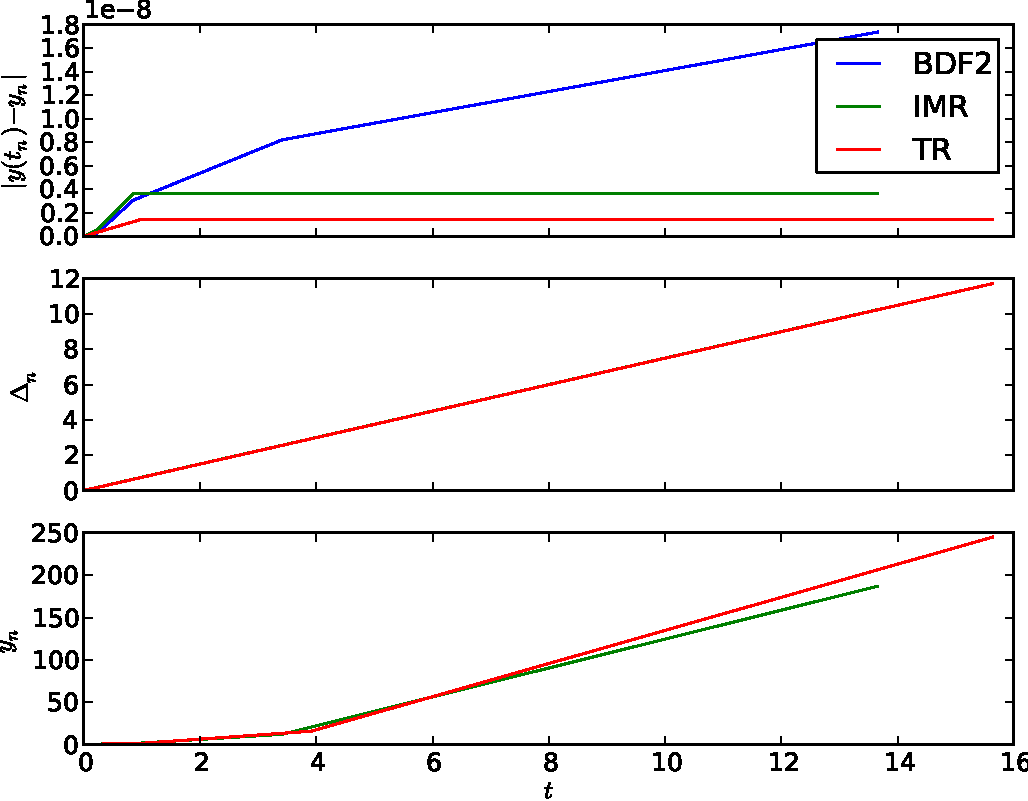
\includegraphics[width=1\textwidth]{plots/aimr_odes/poly2-errornormsvs-dtsvs-tracevaluesvstimes}
  \caption{Absolute error, time step size and computed solutions for the example ODE with exact solution $y(t) = t^2 + 0.5$.}
  \label{fig:imr-poly2-example}
\end{figure}


\subsection{Oscillatory, damped example}
\label{sec:oscill-damp-example}

The next test features a damped oscillatory solution
\begin{equation}
  \label{eqn:imr-test-osc-damp}
  \begin{aligned}
    y(t) &= e^{-\beta t} \sin(\omega t), \\
    f(t,y) &= - \beta e^{-\beta t} \sin(\omega t) + \omega e^{-\beta t} \cos(\omega t).  \end{aligned}
\end{equation} 
The adaptive algorithm should oscillate the step size in time with the oscillating truncation error ($\pd{}{t^3} \sin(t) = -\cos(t)$), while at the same time gradually increasing the step size as the term $e^{-\beta t}$ goes to zero.

??ds write out full lte calculations?

\begin{figure}
  \centering 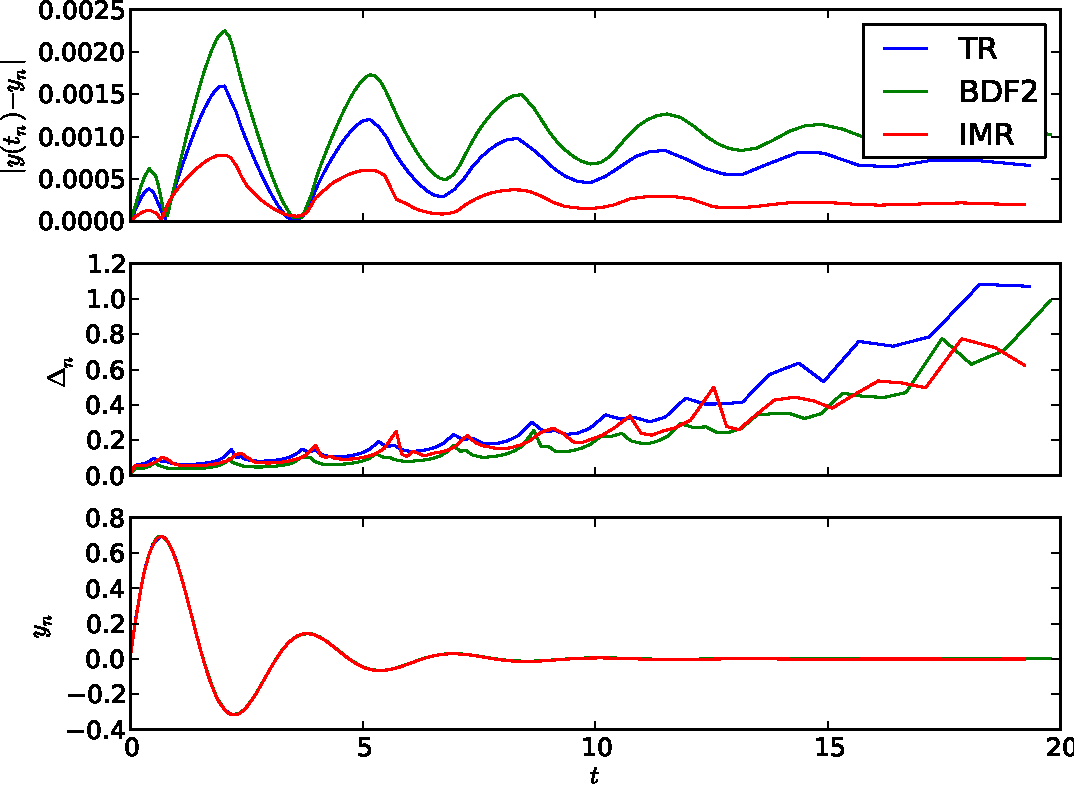
\includegraphics[width=1\textwidth]{plots/aimr_odes/damped_oscillation-errornormsvs-dtsvs-tracevaluesvstimes}
  \caption{Absolute error, time step size and computed solutions for the oscillatory, damped example ODE with exact solution $y(t) = e^{-0.5t} \sin(2\pi t)$.}
  \label{fig:imr-osc-example}
\end{figure}

The ODE was solved with parameters $\omega = 2 \pi$ and $\beta = 0.5$, the results are shown in \cref{fig:imr-osc-example}.
All three methods have similar errors and time step sizes.
The IMR method chooses slightly smaller steps than TR (which probably explains the slightly lower error magnitudes.
BDF2 has the worst errors as expected because its error coefficient is the largest.

Note that the plot shows the global error, whereas local truncation error estimates are used for step size selection calculations.
Hence the fact that the global error increases above the tolerance, $\toltt$, is not surprising.

Interestingly, there is a slight lag on the time step response of the IMR method as time steps become larger.
This could be due to the fact that IMR uses data from three previous steps in its LTE estimate, whereas the others only use two previous steps.

In \cref{fig:imr-osc-example-scatter} we show plots of the decrease in global error norm as the tolerance is decreased. 
The consistent decrease in the error norms indicates that the all of the adaptive methods are able to control the error in the expected manner.
Plots for the example problems the following Sections are very similar and so are not shown.

\begin{figure}
  \centering 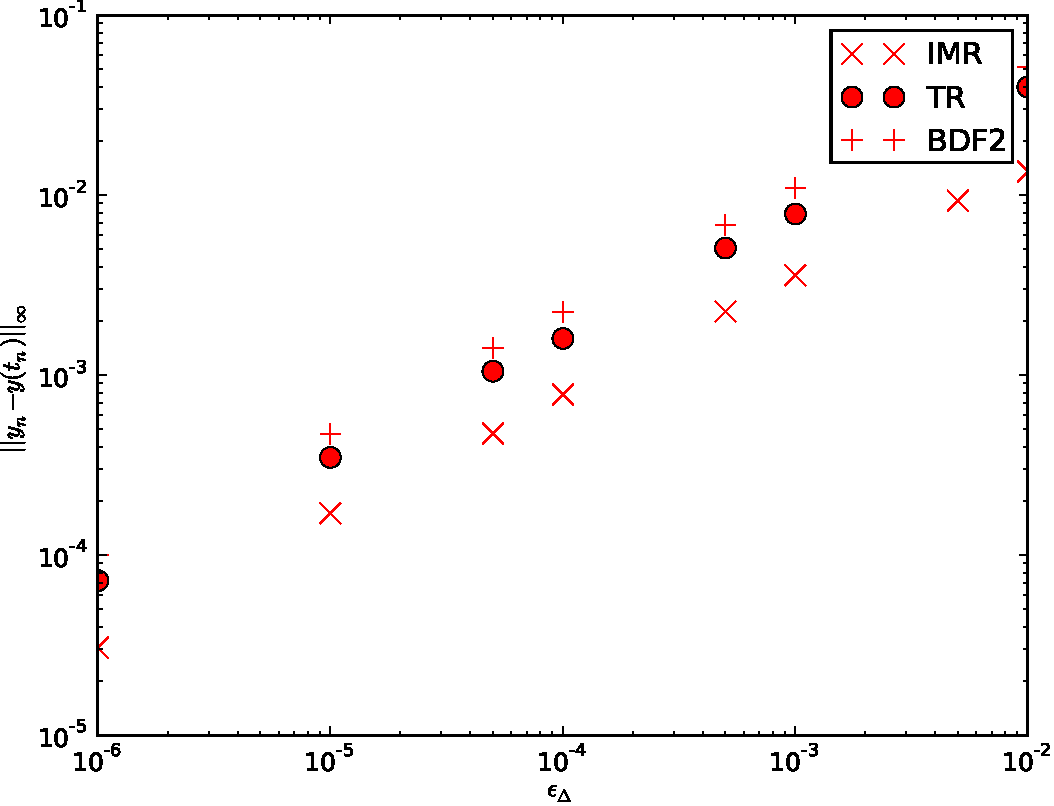
\includegraphics[width=1\textwidth]{plots/aimr_odes/damped_oscillation-maxoferrornormsvs-tol}
  \caption{Behaviour of the global error norm with varying tolerance for the oscillatory, damped example ODE with exact solution $y(t) = e^{-\beta t} \sin(\omega t)$.}
  \label{fig:imr-osc-example-scatter}
\end{figure}

\subsection{Stiff problem}
\label{sec:imr-stiff-example}

We consider stiff example ODE used in the definition of A-stability:
\begin{equation}
  \label{eqn:imr-test-stiff}
  \begin{aligned}
    f(t, \yv) = -\lambda t, \\
  \end{aligned}
\end{equation}
with the exact solution
\begin{equation}
  \label{eqn:imr-test-stiff-exact}
  \yv(t) = e^{-\lambda t} \yv_0. \\
\end{equation} 
This example will test that the single step of the eBDF method provides reliable LTE estimates even in cases of extreme stiffness.
The time steps should start small but rapidly increase as the initial transient decays.

The results of the applying the three methods to problem~\cref{eqn:imr-test-stiff} with $\lambda = 100$ (fairly stiff) are shown in \cref{fig:imr-stiff-example}.
The behaviour of the three time integrators is essentially the same, indicating that our adaptivity algorithm is effective for stiff problems.

\begin{figure}
  \centering
  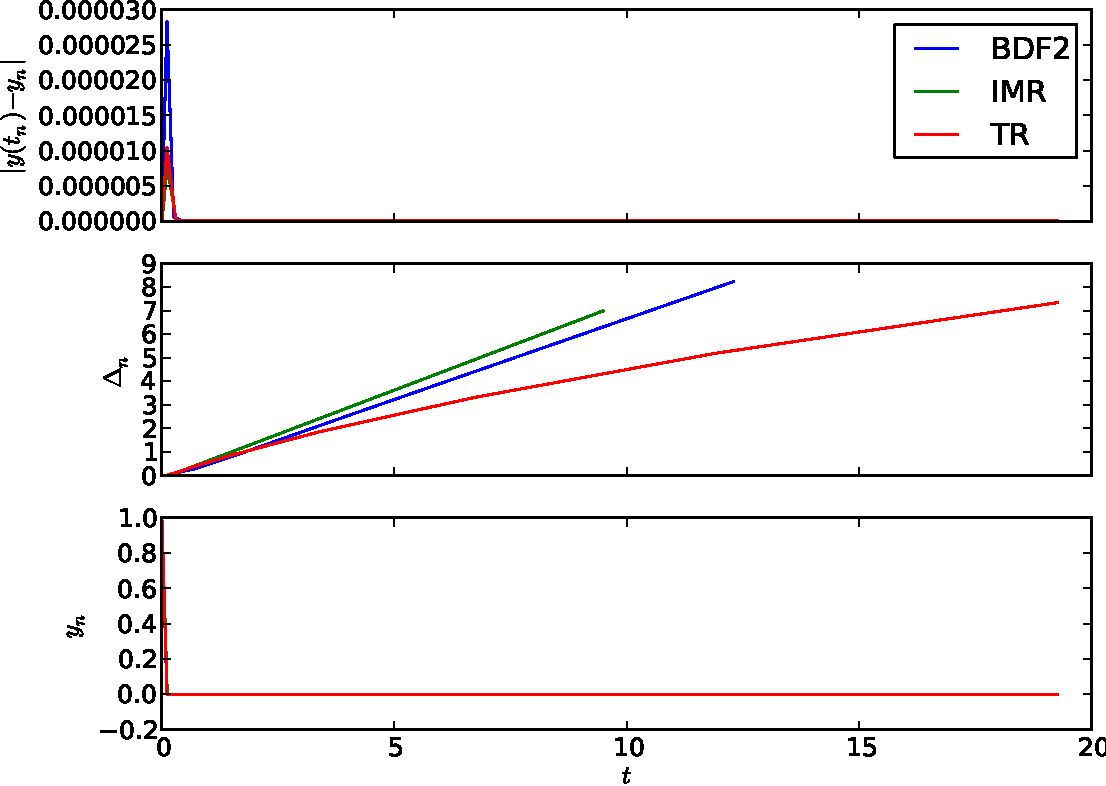
\includegraphics[width=1\textwidth]{plots/aimr_odes/simple_stiff-errornormsvs-dtsvs-tracevaluesvstimes}
  \caption{Absolute error, time step size and computed solutions for the stiff example ODE.}
  \label{fig:imr-stiff-example}
\end{figure}


\subsection{Order reduction example}
\label{sec:order-reduct-example}

\begin{figure}
  \centering  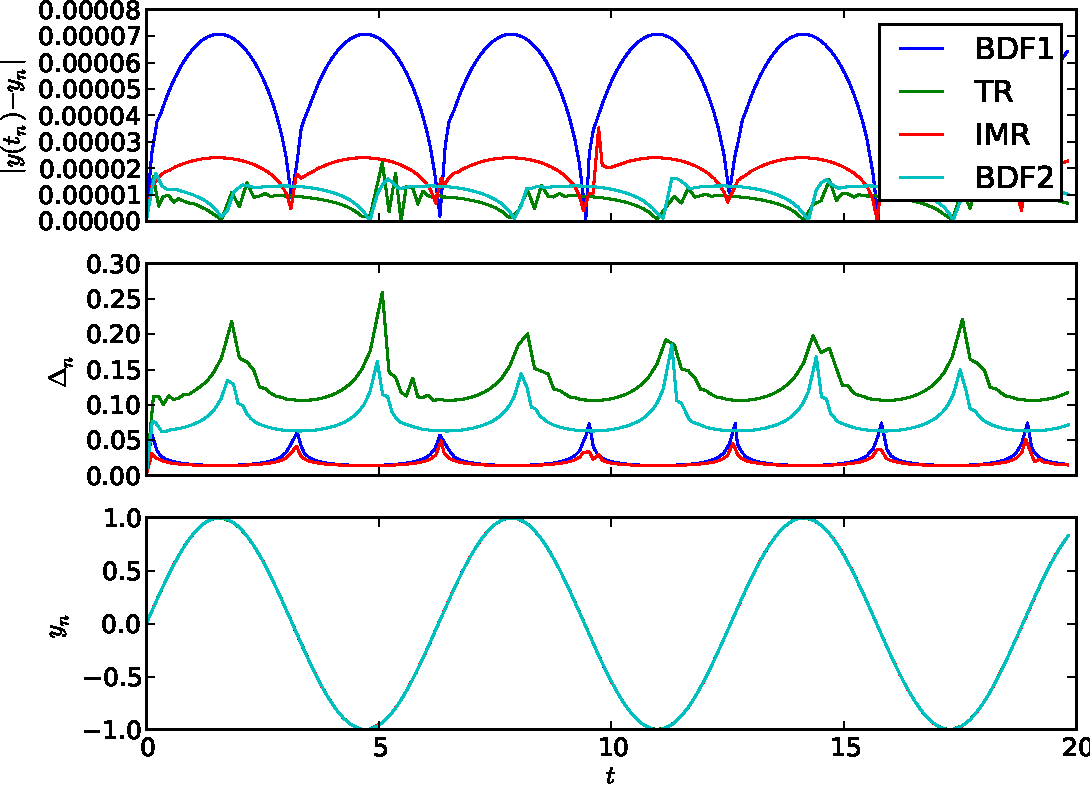
\includegraphics[width=1\textwidth]{plots/aimr_odes/strong_order_reduction-errornormsvs-dtsvs-tracevaluesvstimes}
  \caption{Absolute error, time step size and computed solutions for the stiff order reduction example ODE given in \cref{eqn:imr-test-order-reduction}
    .}
  \label{fig:imr-order-reduction-example}
\end{figure}

\begin{figure}
  \centering  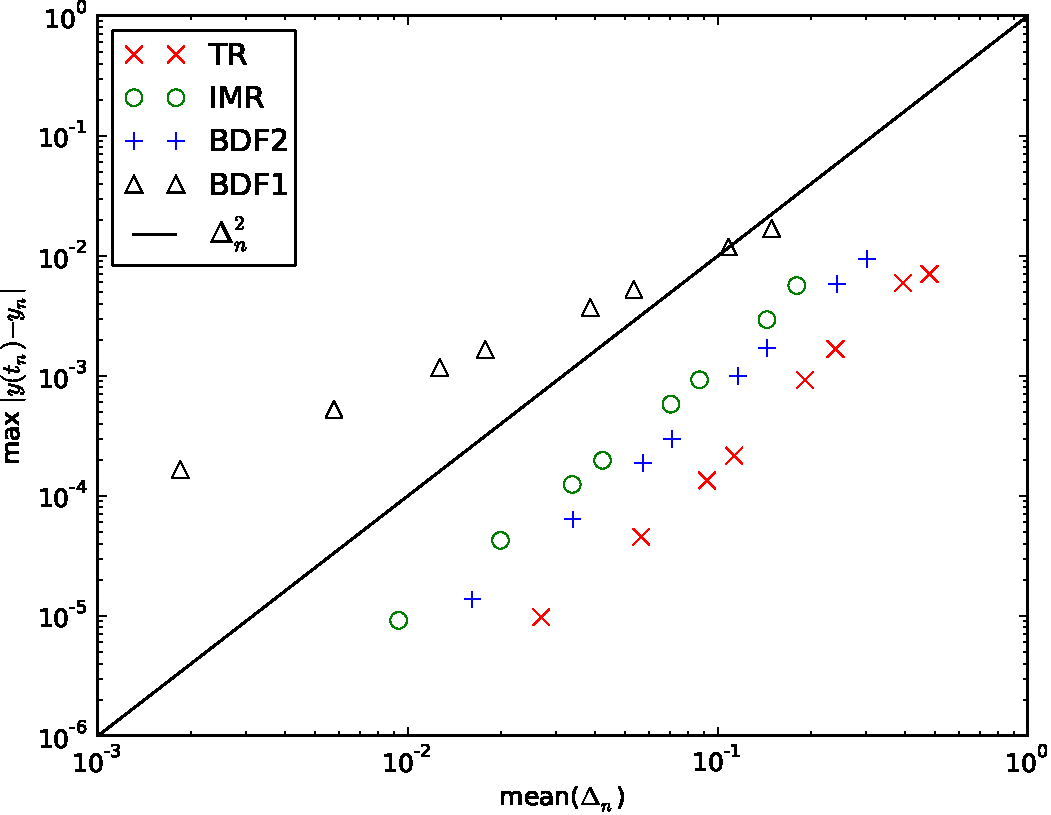
\includegraphics[width=1\textwidth]{plots/aimr_odes/order_reduction-maxoferrornormsvsmeanofdts.pdf}
  \caption{Maximum over time of absolute error vs mean time step for the order reduction example.}
  \label{fig:imr-order-reduction-convergence}
\end{figure}

The order reduction effect should be automatically detected and adjusted for by a good adaptive time step selection algorithm so as a final example we study \cref{eqn:imr-test-order-reduction}, the test ODE for order reduction discussed in \cref{sec:order-reduction}.
For these experiments we chose an oscillatory function, $g(t) = \sin(t)$ and $\lambda = 100$.

So, using \cref{eq:reduced-order-imr-truncation-error}, the dominant term LTE of IMR for the case when $\dtn \gtrsim 0.01$ is
\begin{equation}
  \lte^\imr = \frac{\dtn^2}{4} \sin(\thf),
\end{equation}
for smaller $\dtn$ the $\dtn^3 \cos(t)$ term will gradually become more important.
Note that for TR and BDF2 $\lte \propto \dtn^3 \cos(t)$, while for BDF1 $\lte \propto \dtn^2 \sin(t)$.
Hence we expect to see the adaptive IMR perform similarly to BDF1, and to select much smaller time steps than TR and BDF2 in order to control the larger errors.
To test this we also run the experiment with an adaptive BDF1 (backwards Euler) method using Milne's method for adaptivity.

The results are shown in \cref{fig:imr-order-reduction-example}. 
As expected the implicit midpoint rule selects time step sizes similarly to the first order BDF1 method due to order reduction.
This allows it to retain similar accuracies to the TR and BDF2 methods at the cost of requiring many more time steps.

The convergence of the solution as $\toltt$ is reduced with fixed $\lambda = 100$ is shown in \cref{fig:imr-order-reduction-convergence}.
Note that IMR still displays second order convergence (albeit with a much larger constant error). 
This is because we are not increasing $\lambda$ as we decrease $\toltt$, so we are measuring the normal convergence rather than B-convergence.


\section{Numerical experiments with an ODE form of the LLG}
\label{sec:imr-ode-llg-numer-exper}

\newsubcommand{\swtimeerr}{\mathcal{E}}{\tau}
\newsubcommand{\merr}{\mathcal{E}}{\mv}

In \thisref{sec:imr-ode-llg-numer-exper} we present numerical experiments on a simple LLG problem.
As in \cref{sec:aimr-testing} we compare the performance of the adaptive IMR algorithm developed in \thisref{sec:adaptive-imr} with the adaptive TR and BDF2 algorithms.
Experiments with more complex LLG problems are shown in \cref{cha:numer-experiments}.

\subsection{Problem definition}

To avoid introducing spatial discretisation issues we choose an example problem that can be modelled using only an ODE: the reversal of a ``small'' spherical particle under spatially-uniform applied field.
With this geometry and with uniform initial magnetisation the magnetostatic field can be analytically shown to be $\hms = -\mv/3$ throughout the domain \cite[112]{Aharoni1996}.
This means that the magnetisation remains uniform for sufficiently small spheres such that the increase in exchange energy due to any non-uniformity is larger than the decrease in magnetostatic energy that could be gained by a non-uniform state.

In this case the Landau-Lifshitz form of the Landau-Lifshitz-Gilbert equation \cref{eqn:nd-llg-full} reduces to
\begin{equation}
  \begin{aligned}
    (1 + \dampc^2) \dmdt &= - \mv \times \hv - \dampc \mv \times \bigs{\mv \times \hv}, \\
    \hv &= \happ + \kone (\mv \cdot \ev) \ev.
    \label{eqn:nd-ode-llg}
  \end{aligned}
\end{equation}

To simplify the problem even further we choose $\kone = 0$ and $\happ(t) = [0, 0, -H]$.
In this case an exact solution is available for the time taken for $\mv$ to reach a given angle to the $z$-axis, and for the amount of precession that will take place in that time \cite{Mallinson2000}.\footnote{Actually the solution for the switching time can be easily extended to $\kone \neq 0$ with $\ev = \unitz$ and/or to any $z$-aligned ellipsoid of rotation.
However it is harder to invert the solution to obtain $\theta(t)$ in these cases.}
The exact solution is best expressed in spherical polar notation:
\begin{equation}
  \begin{aligned}
    \theta &= \cos^{-1}(m_z/1),\\
    \phi &= \tan^{-1}(m_y/m_x),
  \end{aligned}
\end{equation}
so $\theta$ is the angle between $\mv$ and the $+z$-direction.
The time for a reversal, $\tau$, from the initial value $\theta_0$ to $\theta$ is given by
\begin{equation}
  \tau(\theta) = t_0 + \frac{\dampc^2 +1}{H \dampc}
  \ln \bigb{ \frac{\tan(\theta/2)}{\tan(\theta_0/2)} }.
  \label{eq:74}
\end{equation}
This allows us to calculate a (global temporal) error in the switching time:
\begin{equation}
  \swtimeerr_n = \abs{t_n - \tau(\theta_n)}.
  \label{eq:sw-time-error}
\end{equation}

Alternatively \cref{eq:74} can be inverted to give $\theta$ as a function of time:
\begin{equation}
  \theta(t) = 2 \tan^{-1} \bigs{ \tan(\theta_0/2) \exp\bigb{\frac{tH\dampc}{\dampc^2 + 1}}}.
\label{eq:77}
\end{equation} 
The azimuthal angle at a given $\theta$ is \cite{Mallinson2000}
\begin{equation}
  \varphi(\theta) = \phi_0 +  \frac{-1}{\dampc} \ln \bigb{ \frac{\tan(\theta/2)}{\tan(\theta_0/2)} }.
\label{eq:78}
\end{equation}
After substituting \cref{eq:77} into \cref{eq:78} and cancelling terms we obtain
\begin{equation}
  \varphi(t) = \phi_0 - \frac{tH}{\dampc^2 + 1}.
  \label{eq:79}
\end{equation}
Hence we can also calculate a (global temporal) error in the magnetisation at time $t_n$
\begin{equation}
  \merr_n = \abs{\mv_n - \mv(t_n)},
\label{eq:m-sphere-error}
\end{equation}
where $\mv(t_n) = \textrm{Cartesian}\bigb{[r=1, \theta=\theta(t_n), \phi=\phi(t_n)]}$.

Which of the error norms $\swtimeerr$ and $\merr$ is most important depends on the aim of the calculation.
We may simply want to find the switching time of the system, in this case the time error norm, $\swtimeerr$, is appropriate (and using time steps such that the precessional behaviour is fully resolved may be excessively expensive).
In other cases an accurate representation of the full behaviour of the system may be needed and $\merr$ is appropriate. 

For the main experiment we choose parameters $H = 1.1$ (sufficient to switch the system) and $\dampc = 0.01$ (roughly the physically relevant value).
We set the initial magnetisation to be just off the $z$-axis in order to avoid a singularity in the reversal time when $\theta_1 = 0$, more precisely $\mv_0 = (0.01, 0.0, 1.0)/\sqrt{1.0001}$. 
The dynamics are simulated for 1000 time units for all simulations, which is sufficient time for the magnetisation to fully switch.

This experiment allows us to check the $\abs{\mv}$ conservation properties of the adaptive IMR, to compare the accuracy of the solution over different time integrators, and to check again that the time step selection is appropriate.

??ds should I do energy conservation? It's a bit complicated: for this example with 0 damping TR and IMR are the same, both seem to give exactly 0 (not 1e-16, actually 0) energy loss. BDF2 has around 1e-14 energy change with no renorm, but around 1e-3 with re-normalisation.

\subsection{Implementation}

The implementation of the three time integration algorithms is exactly as discussed previously except that the TR and BDF2 methods sometimes includes an additional re-normalisation step after each time step to enforce constant $\abs{\mv}$.
The re-normalisation is done by simply replacing $\mv$ by $\mv/\abs{\mv}$, it is carried out after the selection of the next time step.
In the experiments we compare the performance with and without re-normalisation where appropriate.

In the experiments below the LL form \cref{eq:ll-nd-llglike} of the LLG is used for ease of implementation.
Linearisation is carried out using the Newton-Raphson method.
Using the skew operator notation from \cref{sec:llg-jacobian} the Newton-Raphson residual is
\begin{equation}
  \rv = (1 + \dampc^2) \dmdt + \skewm{\mv} \cdot \hv + \dampc \skewm{\mv}\skewm{\mv} \cdot \hv.
\end{equation}
The corresponding Jacobian can be easily derived using the methods discussed in \cref{sec:llg-jacobian} (note that here $\hv \neq \hv(\mv)$), it is:
\begin{equation}
  \Jm = \pd{\rv}{\mv} = (1 + \dampc^2) J_{ts} \Idm_3 - \skewm{\hv} - \dampc \skewm{ \mv \times \hv }
  - \dampc \skewm{\mv} \skewm{\hv}.
\end{equation}

The $3 \times 3$ Jacobian is calculated analytically and inverted using a direct solve.
Unless otherwise specified the Newton tolerance is $\newtontol = 10^{-12}$ and the adaptive integrator tolerance is $\toltt = 10^{-4}$.
The initial time step is $\dtinitial = 10^{-3}$ which is sufficiently small to allow the adaptive algorithm to naturally increase $\dtn$ to an appropriate value.


\subsection{Numerical results}

\begin{figure}
  \centering
  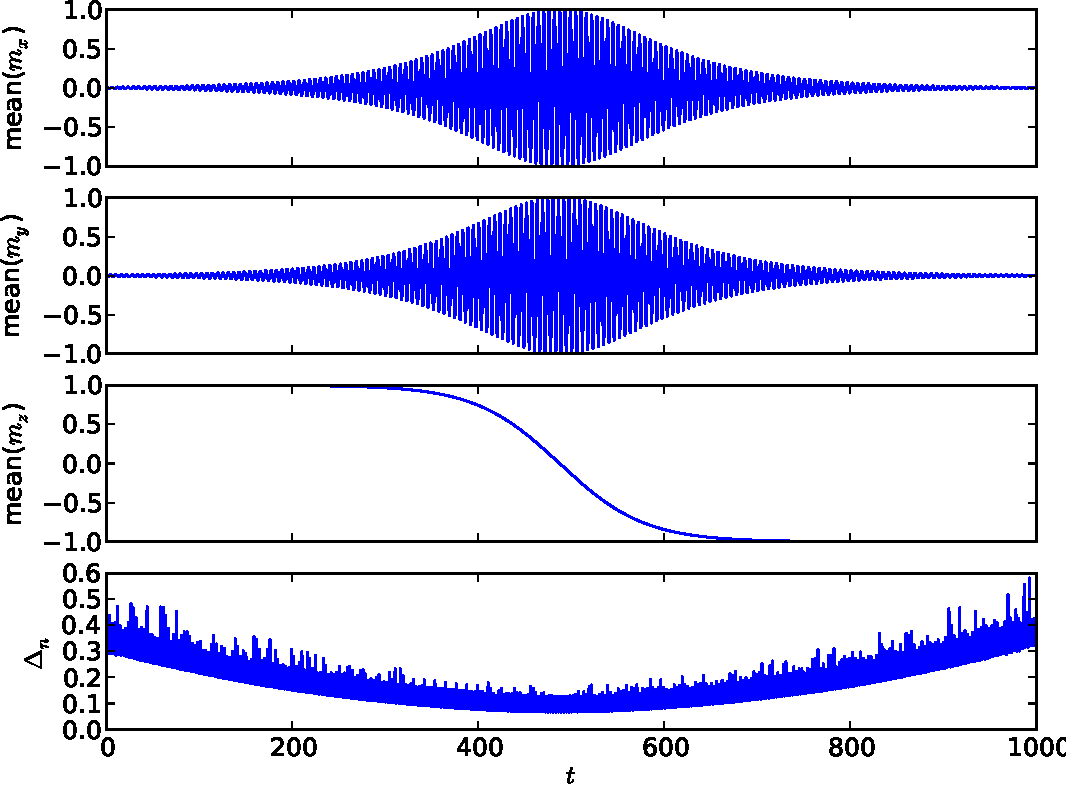
\includegraphics[width=0.8\textwidth]{plots/aimr-sphere-relax/imr0-meanmxsvs-meanmysvs-meanmzsvs-dtsvstimes.pdf}
  \caption{Plot of $\mv$ and $\dtn$ over time for the relaxing nano-sphere problem solved by adaptive IMR.}
  \label{fig:imr-llg-ode}
\end{figure}

The behaviour of the magnetisation and the time step selection using the adaptive IMR algorithm developed in \thisref{sec:adaptive-imr} is shown in \cref{fig:imr-llg-ode}.
The solutions given by adaptive BDF2 and TR (with $\abs{\mv}$ re-normalised after each time step)  are shown in \cref{fig:bdf2-llg-ode,fig:tr-llg-ode} respectively.
The overall behaviour of the IMR time step selection algorithm can be seen to be working as expected: large steps are chosen at the start when very little switching occurs, the step size decreases as switching occurs and finally grows again as the switching finishes.

The origin of the many small peaks in the time step is more difficult to understand.
They have the same period as the precession, but the exact solution for the precession as a function of time, \cref{eq:79}, has no periodic behaviour!
Results for different values of $\dampc$ and $\toltt$ (not shown) show the same behaviour, as do the results for the adaptive TR (\cref{fig:tr-llg-ode}), BDF2 (\cref{fig:bdf2-llg-ode}) and BDF1 (not shown) algorithms.
It is likely that the numerical approximations to the time derivative have some periodicity which does not appear in the exact solution (\cf \cref{sec:order-reduct-example} where the exact solution has no $\lambda$ dependence but the numerical behaviour is strongly affected by $\lambda$).

Note that the accuracy of the switching time given by BDF2 (for the same error tolerances) is terrible.
This is due to BDF2's spurious numerical damping (see \cref{sec:numerical-damping}) which initially moves the solution towards the unstable fixed point at $\mv=[1, 0, 0]$.
The accuracy of the TR solution is (qualitatively) good.
The time steps selected by the three algorithms are qualitatively similar, TR selects slightly larger steps as would be expected due to its lower local truncation error (see \cref{sec:deriv-local-trunc}).


\begin{figure}
  \centering
  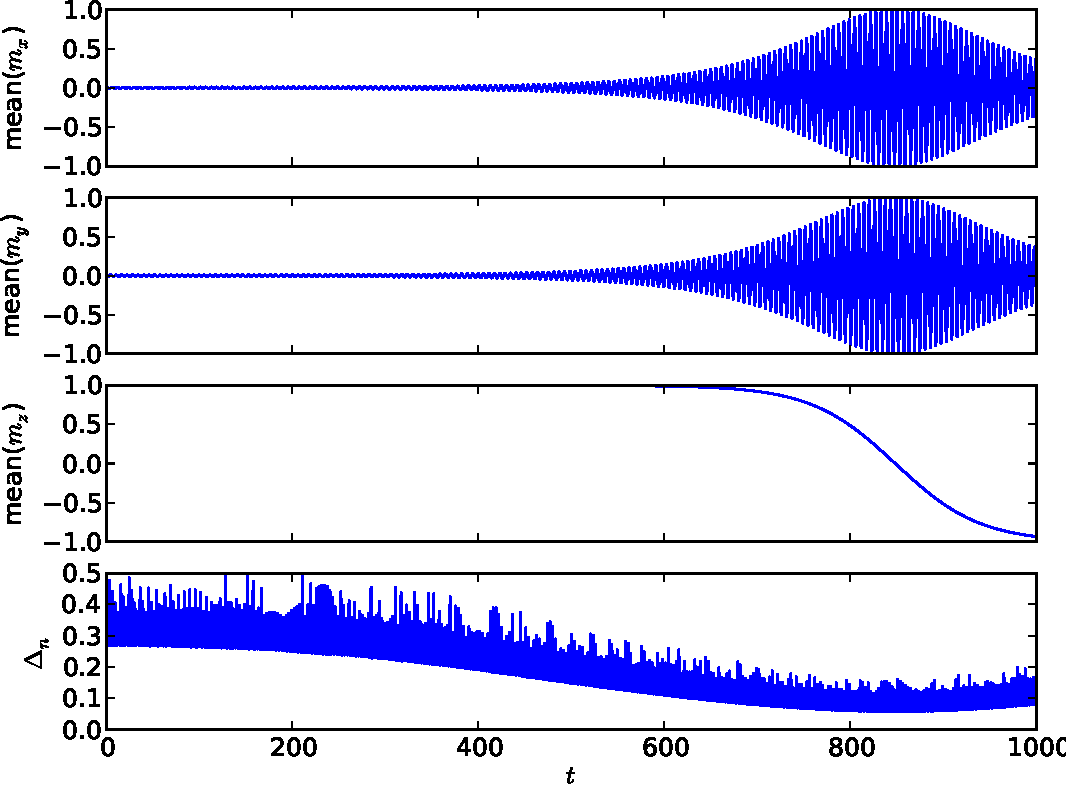
\includegraphics[width=0.8\textwidth]{plots/aimr-sphere-relax/bdf21-meanmxsvs-meanmysvs-meanmzsvs-dtsvstimes.pdf}
  \caption{Plot of $\mv$ and $\dtn$ over time for the relaxing nano-sphere problem solved by adaptive BDF2.}
  \label{fig:bdf2-llg-ode}
\end{figure}


\begin{figure}
  \centering
  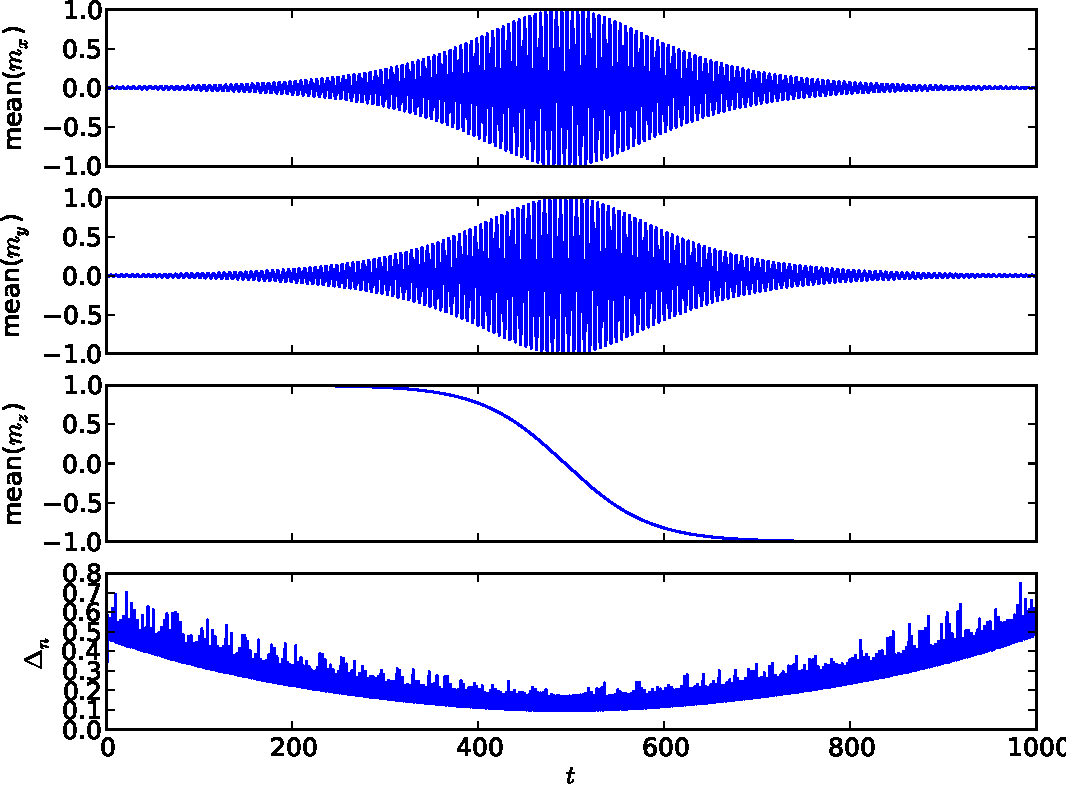
\includegraphics[width=0.8\textwidth]{plots/aimr-sphere-relax/tr1-meanmxsvs-meanmysvs-meanmzsvs-dtsvstimes.pdf}
  \caption{Plot of $\mv$ and $\dtn$ over time for the relaxing nano-sphere problem solved by adaptive TR. ??ds do I need this?}
  \label{fig:tr-llg-ode}
\end{figure}

The behaviour of the magnetisation length over time is shown in \cref{fig:ml-aimr-ode}.
The maximum error is $\abs{\abs{\mv} -1} \approx 10^{-12}$, which is consistent with the Newton tolerance.
This conservation behaviour of IMR does not vary significantly with changes to any parameter other than the Newton tolerance (plots not shown ??ds impossible to show--too many axes... could do a scatter of everything? Too many plots already in this section!).
% ./parameter-sweep.py -p imr_ode_llg -p aimr_ode_llg --clean && parse.py --print-data max-max-ml -d /mnt/moredata/optoomph/user_drivers/micromagnetics/experiments/parameter_sweeps/aimr_ode_llg -f "('-ts', 'imr')" -d /mnt/moredata/optoomph/user_drivers/micromagnetics/experiments/parameter_sweeps/imr_ode_llg

\begin{figure}
  \centering
  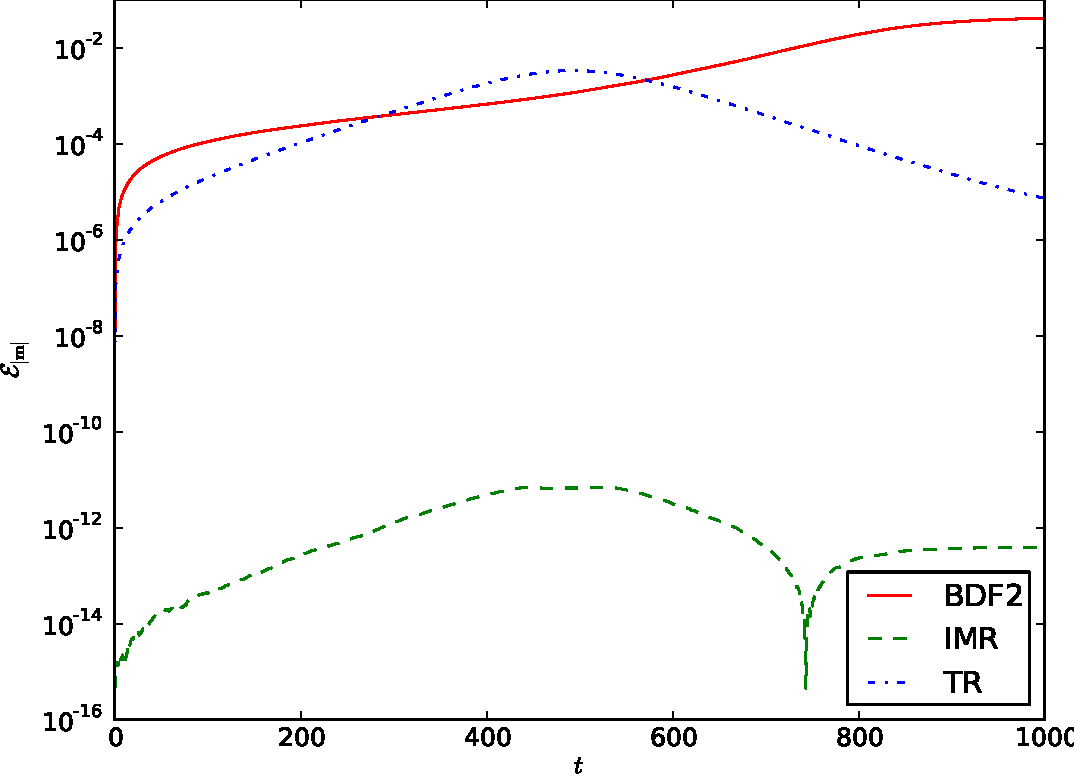
\includegraphics[width=0.8\textwidth]{plots/ode_llg_adaptive_ml/mlengtherrormaxesvstimes}
  \caption{Plot of magnetisation length errors, $\abs{\abs{\mv} -1}$, over time for the relaxing nano-sphere problem solved with each of the three adaptive integrators (without re-normalisation).}
  \label{fig:ml-aimr-ode}
\end{figure}


\begin{figure}
  \centering
  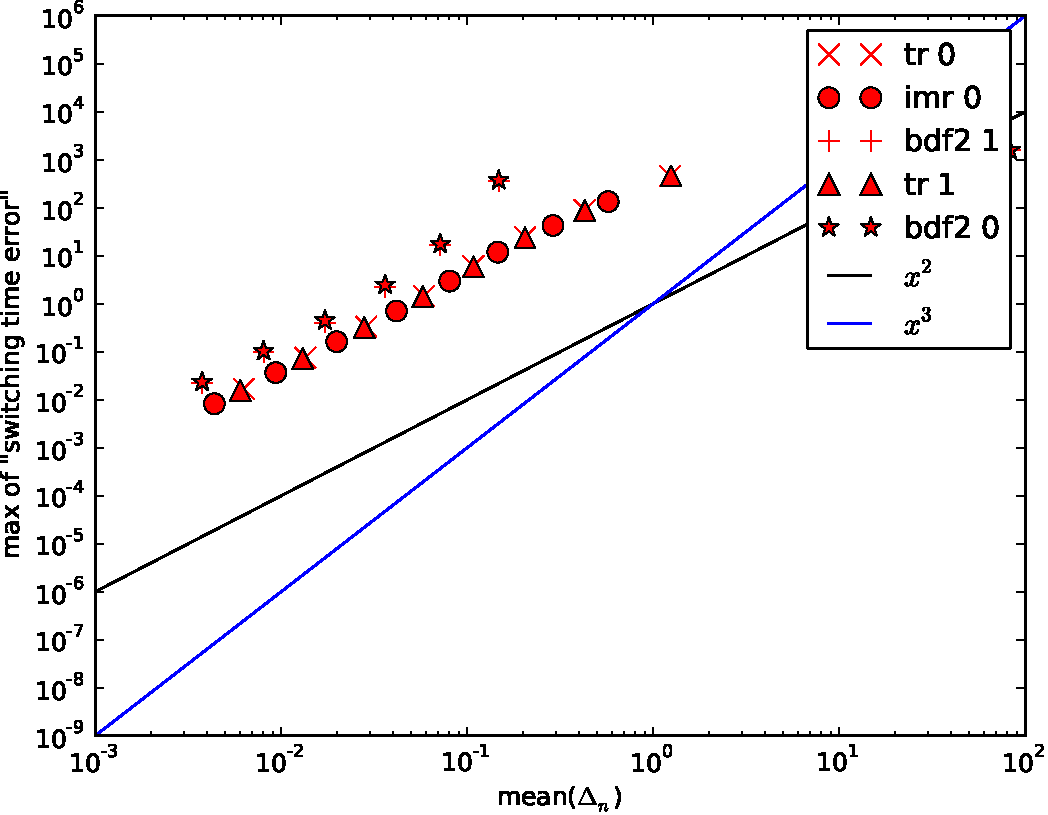
\includegraphics[width=0.8\textwidth]{plots/ode_llg_adaptive_convergence/maxofswitchingtimeerrorvsmeanofdts}
  \caption{Convergence plots of the switching time error, \cref{eq:sw-time-error}, against average time step for constant step IMR, adaptive IMR, adaptive TR and adaptive BDF2. ??ds zoom in, remove guidelines, Better legend}
  \label{fig:llg-ode-convergence-swtime}
\end{figure}


Finally we show convergence plots with respect to the two error norms.
\Cref{fig:llg-ode-convergence-swtime,fig:llg-ode-convergence-m} show the convergence with respect to the switching time error and total error respectively.
Adaptive TR and BDF2 algorithms both with and without re-normalisation of the magnetisation after
each step are shown, along with the adaptive IMR algorithm developed in \thisref{sec:adaptive-imr}.


In \cref{fig:llg-ode-convergence-swtime} (switching time error) the convergence lines for TR and IMR are flat as would be expected, BDF2 does not attain this asymptotic convergence state until a comparatively small time step.
The maximum errors are around $1000$ time units, a relative error of $\sim 1$.
The errors of TR and IMR are extremely similar for a given mean time step size.
Once the asymptotic convergence regime is reached BDF2 has roughly triple the error of the other methods.
Note that the re-normalisation of $\mv$ in BDF2 and TR has only a minimal effect on their global error, this indicates that length conservation property of IMR is unlikely to be providing a major benefit to the global error in this simple example.


In \cref{fig:llg-ode-convergence-m} (overall error) the convergence lines show a kink around $\mean(\dtn) = 0.1$.
This is because $\abs{\mv} \approx 1$ and so the error norm $\merr$ cannot be worse than the anti-parallel case.\footnote{A more effective error norm for such large error cases would be to use polar coordinates and track the total azimuthal angle passed through during the simulation. However 1) this is non-trivial to implement in general; 2) some rescaling would be required to prevent the $\varphi$ error contribution from dominating that of $\theta$; and 3) we are not very interested in cases where the solution is highly inaccurate anyway.}
Above the kink the azimuthal angle is inaccurate and so the error norms are meaningless, below the kink the usual convergence behaviour can be seen.
The comparing the error norms different methods we see the same relationships as for \cref{fig:llg-ode-convergence-swtime}: BDF2 has triple the error and re-normalisation has little effect.


Note that TR consistently chooses large time steps than IMR despite both measures of the global error being very similar.
This may be due to differing accuracies in the estimation of the LTE.
Alternatively LTE of IMR may be somewhat larger (as expected), with the geometric integration properties of IMR reducing the build up of global error.


Note that there are fewer visible points on \cref{fig:llg-ode-convergence-swtime,fig:llg-ode-convergence-m} for BDF2 than the other two methods, this is because at larger tolerances BDF2 takes overly large time steps (and has large global errors to match).
Hence some points for BDF2 do not fit on the same scale (for these missing points: $\mean(\dtn) \approx 10\dash 100$, $\swtimeerr \approx 1000 \approx$ \ie a relative error of 1, $\merr \approx 2$).
This is consistent with the quantitatively wrong results given by BDF2 in \cref{fig:bdf2-llg-ode}.

\begin{figure}
  \centering
  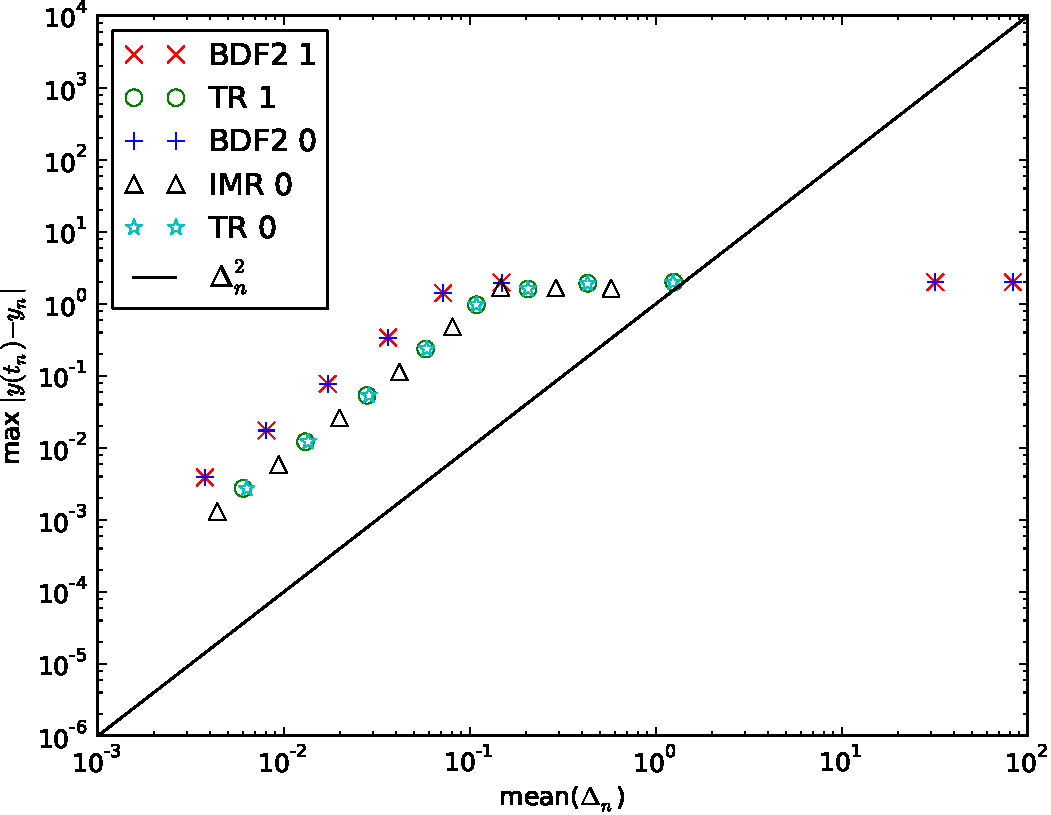
\includegraphics[width=0.8\textwidth]{plots/ode_llg_adaptive_convergence/maxoferrornormsvsmeanofdts}
  \caption{Convergence plots of the error in magnetisation, \cref{eq:m-sphere-error}, against average time step for constant step IMR, adaptive IMR, adaptive TR and adaptive BDF2. ??ds zoom in, remove guidelines, Better legend}
  \label{fig:llg-ode-convergence-m}
\end{figure}

\section{Conclusions}

We have implemented an efficient algorithm for adaptive time step selection with the implicit midpoint rule.
The algorithm has been tested on a number of ODEs and found to choose similar time steps to other second order time integrators.
It has also been shown to be robust in stiff problems and to control the error effectively even when order reduction phenomena are encountered.

When applied to an ODE form of the LLG the adaptive IMR algorithm conserves $\abs{\mv}$ as expected.
It also appears to give slightly smaller global error norms than would be expected from its local truncation error, this may be due to the geometric integration properties.
Any effects of these geometric integration properties would be expected to be greatly amplified when solving ODE problems with many interacting spins or PDE problems.
This will be tested in \cref{cha:numer-experiments} where the adaptive IMR algorithm is combined with the PDE methods discussed in other chapters.


%%% Local Variables:
%%% mode: latex
%%% TeX-master: "./main"
%%% End:
